\chapter{Introduction} 
\label{chp:intro}

Modern robot technologies serve a wide range of applications. 
%
As a result, the human society is now experiencing benefits brought by the robot technology more than ever before.
%
For example, in factories, millions of industrial robots operating the production line enormously boosted the productivity; 
in hospitals, surgery robots help doctors to achieve high accuracy in the surgical procedures; 
meanwhile, in military and agricultural applications, unmanned systems, such as drones, are widely deployed for the aerial surveillance.


%
One power that pushes the robotics research forward is the progress of the sensing and computing technologies. 
%
Sensing ability is critical for robots to know about their environments. 
According to Siegwart, Nourbakhsh, and Scaramuzza, sensors can be classified as proprioceptive/exteroceptive sensors or passive/active sensors using two important function axes~\cite{SieNouSca11}.
%
Proprioceptive sensors such as odometers,
compass, measure internal values to the robot, for example, motor speed, orientation, joint angles, etc.
%
Exteroceptive sensors such as cameras, laser range-finders, acquire the information from the robot's environment, for example, the distance between a robot to an obstacle, or the light intensity. 

%
We have observed a great success has been achieved in the areas of robot perception, motion/path planning, localization and mapping, etc. 
%
However, in practice, even the most advanced sensing technique cannot guarantee to produce a perception of the
environment without any uncertainty.  
%
Thus, to solve those difficult robotics problems such as planning or SLAM, etc., we must process the uncertainty from sensing and motion properly.
%
A primary question is about how does a robot represent and reason about its perceived information with uncertainty.
%
Therefore, the first goal of this dissertation is studying a planning algorithms with constraints on the robot's sensing and computing ability.

\subsection{Geometric Planning Algorithm}
We consider a problem that given a robot, equipped with exteroceptive sensors,
has limited sensing and computing
ability and a known planar environment in which the landmarks are
placed. 
We mainly focus on how to model the robot's perception using simple
geometric structures.
We also consider how to make effective plans for the robot to complete certain navigation tasks 
in spite of a noisy perception.

We have borrowed an idea of using the set-based representations of uncertainty to describe the robot's knowledge of
itself and the environment, from the work of O'Kane and LaValle~\cite{OKaLav08,Lav06}, and Erdmann and Mason~\cite{ErdMas88}. 
The key is maintaining a set, called information state (\textit{I-state}), of ``possible states'' that are consistent with the robot's
history of actions and observations. 
The robot can plan a series of movements in terms of its I-state. 
Generally, the procedures of maintaining an I-state are
computationally expensive. 
We have contributed to a computationally
inexpensive approach, called ``constrained geometric
approximation'' (CGA), for the robot to maintain an ``over-approximation'' of its true
I-state.

The preliminary version of the constrained geometric approximation method was
introduced by O'Kane's work~\cite{OKa11}, where a set of rectangles
were effective to maintain proximity of unpredictably moving targets. 
Here our 
contributions include (1) formulating the operations required to constrain the
approximation in a fixed range space, and (2) introducing a new type of range
space called ``double rectangle space'' to increase the approximation accuracy, especially in the environments with numerous non-convex objects (Figure~\ref{fig:nav-clutter}), 
and (3) conducting a series of experiments, and evaluating the performance of
our approach using different types of range spaces, by measuring the computation time,
the approximation quality, and the task completion rate.

\begin{figure}
  \centering
  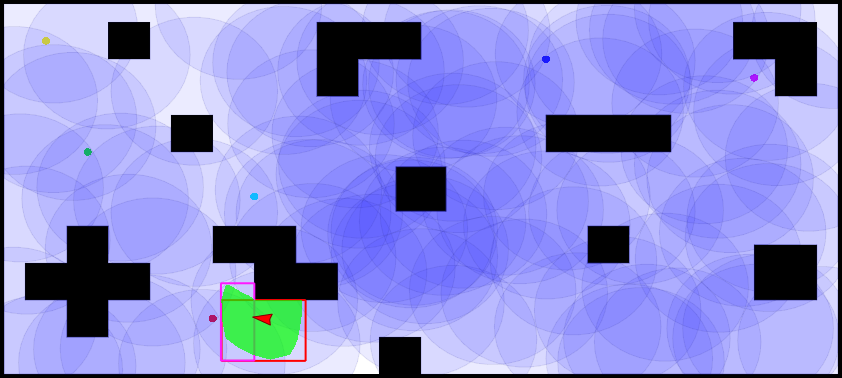
\includegraphics[width=.9\columnwidth]{figs/dbrect_clutter.png}
  \caption{A robot (red arrow) navigates itself in an environment with obstacles (black) and landmarks.
    The blue circles are the ranges in which the robot receive observations from the landmarks.
    The green region denotes the robot's true information state. 
    A union of two red boxes represents an over-approximation
    of the information state using double-rectangle.}
  \label{fig:nav-clutter}
\end{figure}

\subsection{Multi-Robot Formation}

As modern robotic research and technology arise, advances and new challenges
involve not only single robots but also large systems of robots. 
Needless to say, well-collaborated work often enhances the effectiveness, flexibility and
fault-tolerance of a single entity. 
A vivid example is shown in the movie ``Big Hero 6'', in which many small robots can configure and re-shape themselves to different formations to accomplish different tasks.
Hereby, research about multi-robot systems, on ground, or in aerial, or under water, attracts a growing number of attentions in recent years\cite{CaoFukKahMen95, DudJenMilWil96, BahSoySah03}. 
Groups of autonomous robots could be used for tasks ranging from exploring and mapping in an unknown environment to deploying large-scale mobile sensor network. 
However, in contrast to a single robot, the multi-robot systems normally raise more complicated problems, such as multi-sensor data fusion in the sensing procedure, or multi-robot collision
avoidance in the motion procedure and multi-robot coordination in the decision-making procedure.

We first describe a novel distributed algorithm that enables a group of mobile
robots to establish an arbitrary formation, including the repeated lattice
pattern, such as the geometric shapes of squares, hexagons, octagons, etc.
Figure~\ref{fig:octsq-init-final} shows an example in which $100$ robots formed 
a repeating octagon-square lattice pattern from a random initial distribution.
\begin{figure}
  \centering
  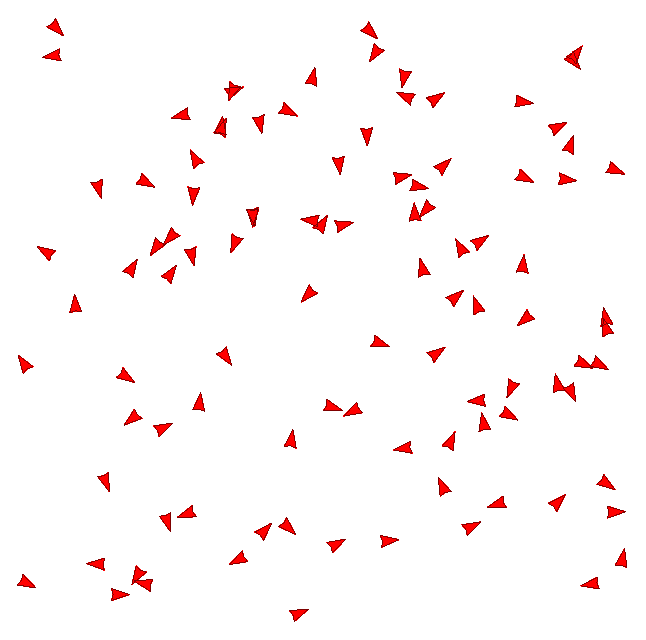
\includegraphics[width=.4\columnwidth]{figs/initial-formation}
  \bigskip
  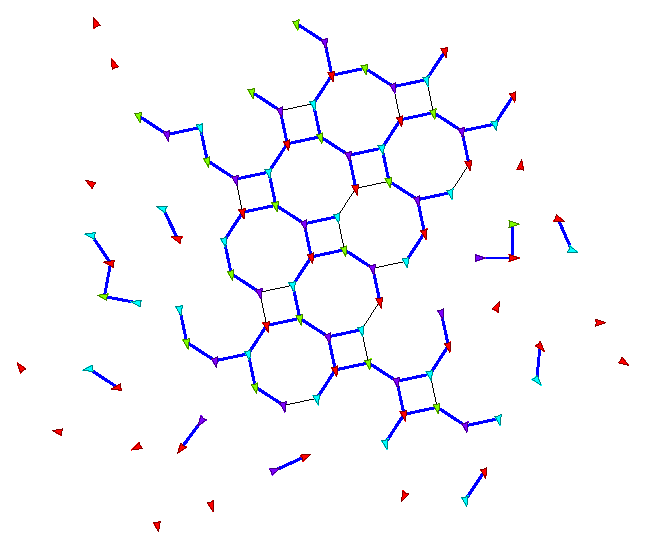
\includegraphics[width=.45\columnwidth]{figs/final-formation}
  \caption{[left] The initial poses of $100$ robots, randomly generated with a
  uniform distribution. [right] The final formation after executing our
  algorithm using the octagon-square lattice graph as an input.}
  \label{fig:octsq-init-final}
\end{figure}
We consider the multi-robot formation problem in a combination of the task
assignment problem~\cite{Kuh55, Mun57} and a graph matching
problem~\cite{Lov86}. Therefore, the major contributions of our work include (1)
a general graph representation of desired formation, called ``lattice graph'',
(2) a novel scheme called ``authority'' to organize the robots into a
globally rooted tree structure, which serves for the local task assignment, 
and (3) a series of experiments to verify the effectiveness of our algorithm.

However, the above-mentioned formation algorithm has two critical limitations.
\begin{enumerate}
\item There is no guarantee that the robots will eventually form the
  desired formation and terminate the algorithm. 
  Instead, the robots may oscillate under some conditions.
\item The motion strategy may cause some robots become
  disconnected with others (Figure~\ref{fig:octsq-init-final}), 
  thus, would decrease the overall solution quality.
\end{enumerate}

To resolve these limitations, we have developed a new scheme by introducing a new communication protocol and a new motion strategy. 
In contrast to the prior algorithm which allocates multiple robots local destinations simultaneously,
the key idea of our new algorithm is relocating only one robot to a position to form the desired pattern sequentially.
Moreover, we have proved the correctness of our formation algorithm: (1) the
output of the algorithm correctly matches the goal lattice pattern, (2) the
algorithm has a time-bounded performance and improved final formation quality, 
compared with the results using the prior formation algorithm.

Chapter~\ref{chp:cga} describes the constrained geometric approximation method 
including: the review of the state-of-the-art,
the problem statement along with the fundamental knowledge related with the
information state, the detail of the algorithm, the experimental results, and conclusions.

In Chapter~\ref{chp:mrf}, we introduce the fundamental concepts of the multi-robot lattice formation problem we want to solve. 
% 
First we overview the related work. 
%
Then we address the problem by defining the robot model, the graph representation of the algorithm input, and the evaluation criteria for the algorithm output. 

Chapter~\ref{chp:mrf1} presents the framework of our primary stateless, task-assignment-based formation algorithm. 
%
We explain the definition of the robot authority and then describe the distributed task-assignment strategy in detail.
%
Also, we illustrate the experiments setup and conclude the method according to the simulation results.

Chapter~\ref{chp:mrf2} extends our discussion about the multi-robot lattice formation problem in Chapter~\ref{chp:mrf}, but focuses on a new decentralized algorithm. 
First we outline the limitations of the prior algorithm, then describe the detail of our new contributions.
Furthermore, we show the proof of the algorithm correctness and the execution time bound.
We also compare the experimental results of both algorithms, and conclude the new methods.

Finally, we give a comprehensive summary of this dissertation in Chapter~\ref{chp:conc}.
